% Provenance (never printed): old terminale S material on the transformation of
% rocks in mountain belts and subduction zones (pressure, temperature, index
% minerals and the Al2SiO5 polymorphs, foliation, contact and regional
% metamorphism). Owner (Sync 0): metamorphism, lithostatic pressure, polymorph,
% index mineral/isograd/metamorphic grade, foliation/schistosity, contact and
% regional metamorphism/aureole. Blueschist and eclogite are g11.06's, the
% geotherm g11.03's, minerals and silicates g11.07's, the rock families, marble
% and slate Book 1's (g6), pressure physics': recalled, never redefined. The
% P-T diagram: figdata/grade-12/al2sio5.py (Holdaway and Mukhopadhyay 1993,
% Table 11; geotherms from Earle 7.3).
\chapter{कायांतरित चट्टानें}\label{ch:g12:metamorphic-rocks}

किसी समुद्री तली पर पंक की एक परत बैठती है और कठोर होकर शेल बन जाती है। उसे कुछ
किलोमीटर नीचे दबा दीजिए और भींचिए, तो वह स्लेट बन जाती है, एक ऐसी चट्टान जो
छत की पतली, समतल पट्टियों में फटती है। उसे और गहरे और गरम में दबाइए, तो उसके नन्हे
शल्क चमचमाते अभ्रकों में बढ़ जाते हैं, जिनके बीच लाल गार्नेट फूलते हैं: एक शिस्ट।
और भी गहरे और गरम में, उसके खनिज स्वयं को हल्की और गहरी
पट्टियों में छाँट लेते हैं: एक नाइस। रास्ते में कुछ भी नहीं पिघला। वही पंक, उन्हीं
रासायनिक तत्त्वों के साथ, बस अपने खनिजों को उस स्थान के अनुरूप फिर से गढ़ता गया जहाँ वह
था। उलटी ओर से पढ़ें, तो किसी कायांतरित चट्टान के खनिज दर्ज करते हैं कि वह स्थान कितना गहरा
और कितना गरम था, और यह अध्याय उन्हें पढ़ना सीखता है।
% ledger: earle:foliation, earle:settings

\begin{recall}
चट्टानें तीन परिवारों में बँटती हैं --- आग्नेय, अवसादी, कायांतरित --- और
शैल-चक्र एक को दूसरे में बदलता है; संगमरमर चूना पत्थर से बनता है और
स्लेट शेल से, बिना पिघले (पुस्तक 1, कक्षा 6)। खनिज एक प्राकृतिक
ठोस है जिसका एक निश्चित रासायनिक संघटन और परमाणुओं की एक क्रमबद्ध
व्यवस्था होती है; भूपर्पटी के अधिकांश खनिज \omterm{def:g11:minerals:silicate}{सिलिकेट} हैं
(\cref{ch:g11:minerals})। \omterm{def:g11:lithosphere-asthenosphere:geotherm}{भूतापीय वक्र} किसी स्थान के नीचे गहराई के सापेक्ष तापमान का
वक्र है; सतह के निकट तापमान प्रति किलोमीटर 25 से
\qty{30}{\celsius} बढ़ता है (\cref{ch:g11:lithosphere-asthenosphere})।
\omterm{def:g11:subduction-zones:subduction}{क्षेपण क्षेत्र} में, ठंडी रहते हुए नीचे ले जाई गई \omterm{def:g11:ocean-ridges:oceanic-lithosphere}{महासागरीय भूपर्पटी}
\omterm{def:g11:subduction-zones:eclogite}{नीलशिस्ट} में, फिर \omterm{def:g11:subduction-zones:eclogite}{एक्लोजाइट} में बदल जाती है (\cref{ch:g11:subduction-zones})।
दाब एक बल है जिसे उस क्षेत्रफल से भाग दिया गया हो जिस पर वह दबाता है; उसे
पास्कल में मापा जाता है, \qty{1}{Pa} = \qty{1}{N/m^2}।
\end{recall}
% ledger: usgs:metamorphic (Book 1 row), webmineral:formulas, earle:settings, earle:controls

\section{ठोस अवस्था में रूपांतरित}

\begin{definition}[कायांतरण]\label{def:g12:metamorphic-rocks:metamorphism}
\emph{कायांतरण}\index{कायांतरण} किसी चट्टान के खनिजों और \omterm{def:g11:igneous-rocks:texture}{गठन} का ठोस अवस्था में
रूपांतरण है, जब उसे ऐसे तापमान और दाब पर लाया जाता है जो उन तापमान और दाब से भिन्न हों
जिनमें वह बनी थी।
उससे बनने वाली चट्टान कायांतरित चट्टान है।
\end{definition}
% ledger: tulane:metamorphism, earle:controls

\omterm{def:g12:metamorphic-rocks:metamorphism}{कायांतरण} जिस चट्टान से शुरू होता है, वह उसकी \omterm{def:g10:soil-formation:weathering-profile}{जनक चट्टान} है, वही शब्द जो
किसी मृदा के नीचे की चट्टान के लिए हैं (\cref{ch:g10:soil-formation})। \omterm{def:g12:metamorphic-rocks:metamorphism}{कायांतरण} लगभग \qty{200}{\celsius} पर शुरू होता है; उससे नीचे,
दबे हुए अवसाद के धीमे परिवर्तन उसके कठोर होकर चट्टान बनने के अंग हैं। वह
वहाँ समाप्त होता है जहाँ चट्टान पिघलने लगती है: उसके बाद जो होता है, वह आग्नेय है। इन
सीमाओं के बीच, हर खनिज तापमान और दाब के केवल एक निश्चित परास में
स्थायी है। उदाहरण के लिए, अधिकांश \omterm{def:g10:soil-formation:clay}{मृत्तिका खनिज} केवल लगभग 150 या
\qty{200}{\celsius} तक टिकते हैं; उससे ऊपर वे अभ्रकों में बदल जाते हैं। जब
परिस्थितियाँ बदलती हैं, तो अस्थायी खनिजों के परमाणु स्वयं को, कण-दर-कण,
ऐसे खनिजों में पुनर्व्यवस्थित करते हैं जो नई परिस्थितियों में स्थायी हों।
% ledger: tulane:metamorphism, earle:controls

परिणाम को चार चीज़ें नियंत्रित करती हैं। \textbf{\omterm{def:g10:soil-formation:weathering-profile}{जनक चट्टान}} रासायनिक
तत्त्व देती है: केवल कैल्साइट से बना चूना पत्थर केवल कैल्साइट से बना
संगमरमर ही बन सकता है। \textbf{तापमान} और \textbf{दाब} तय करते हैं कि कौन-से
खनिज स्थायी हैं। और \textbf{जल}, जो कणों के बीच थोड़ी मात्रा में मौजूद होता है,
घुले हुए आयनों को एक कण से अगले तक ले जाता है और अभिक्रियाओं को तेज़
करता है। \omterm{def:g12:metamorphic-rocks:metamorphism}{कायांतरण} धीमा है: नए खनिज एक मिलियन वर्ष में लगभग एक मिलीमीटर बढ़ते
हैं। चट्टानों को दबाने वाली विवर्तनिक घटनाएँ भी धीमी होती हैं, इसलिए
अभिक्रियाओं को प्रायः पूरा होने का समय मिल जाता है।
% ledger: earle:controls

\subsection{ऊपर की चट्टानों का भार}

गहराई $z$ पर दबी चट्टान अपने ऊपर की सारी चट्टान का भार उठाती है।

\begin{definition}[शैलस्थैतिक दाब]\label{def:g12:metamorphic-rocks:lithostatic}
गहराई $z$ पर \emph{शैलस्थैतिक दाब}\index{शैलस्थैतिक दाब}
वह दाब है जो किसी चट्टान पर उसके ऊपर की चट्टान के स्तंभ का भार डालता
है। वह सभी दिशाओं में समान होता है।
\end{definition}
% ledger: earle:controls (confining pressure, equal in all directions), tulane:metamorphism

\begin{proposition}[शैलस्थैतिक दाब]\label{prop:g12:metamorphic-rocks:lithostatic}
एकसमान घनत्व $\rho$ वाले चट्टान के स्तंभ के नीचे, \omterm{def:g12:metamorphic-rocks:lithostatic}{शैलस्थैतिक दाब}
गहराई $z$ पर यह है:
\[
  P = \rho g z ,
\]
जहाँ $g$ गुरुत्वीय त्वरण है; वायुमंडल का
दाब, लगभग \qty{0.1}{MPa}, नगण्य माना गया है।
\end{proposition}

\begin{proof}
क्षैतिज अनुप्रस्थ काट $A$ वाला चट्टान का एक ऊर्ध्वाधर स्तंभ लीजिए, सतह से
गहराई $z$ तक। उसका आयतन $Az$ है, उसका द्रव्यमान $\rho A z$, और
उसका भार $\rho A z g$। यह भार स्तंभ के तल पर क्षेत्रफल $A$ पर टिका है,
इसलिए वहाँ दाब $P = \rho A z g / A = \rho g z$ है।
\end{proof}

\omterm{def:g12:continental-crust:continental-crust}{महाद्वीपीय भूपर्पटी} के माध्य घनत्व, $\rho = \qty{2830}{kg/m^3}$,
और $g = \qty{9.81}{m/s^2}$ के साथ दाब प्रति मीटर $\rho g = 2830 \times 9.81
\approx \qty{27800}{Pa}$ बढ़ता है, यानी प्रति किलोमीटर लगभग \qty{27.8}{MPa}।
\qty{35}{km} मोटी भूपर्पटी के आधार पर वह इस मान तक पहुँचता है:
\[
  P = 2830 \times 9.81 \times \num{35000} \approx \qty{9.7e8}{Pa} \approx
  \qty{0.97}{GPa},
\]
लगभग \qty{1}{GPa}: समुद्र-तल पर वायुमंडल के दाब का लगभग दस हज़ार गुना।
दाबों को अक्सर उलटी ओर से, गहराइयों के रूप में, पढ़ा जाता है:
\qty{1}{GPa} का दाब $\num{e9}/(2830 \times 9.81) \approx \qty{36}{km}$ की
गहराई पर पहुँचता है।
% values: P_35km_gpa 0.97168, dPdz_mpa_per_km 27.762, z_1gpa_km 36.02 (al2sio5.py)
% ledger: cm95:crust; Book 1: ussa76:sea-level (101 325 Pa, g0 = 9.80665 m/s2)

चट्टानों का भार सभी ओर से समान रूप से दबाता है। किसी पर्वत-पट्टी में
प्लेटें एक दिशा में धक्का जोड़ देती हैं: चट्टान ऊपर की अपेक्षा किनारों से
अधिक ज़ोर से भींची जाती है। यह \emph{दिष्ट} दाब यह नहीं बदलता कि कौन-से
खनिज स्थायी हैं, पर यह बदलता है कि वे कैसे व्यवस्थित होते हैं, जैसा
\cref{sec:g12:metamorphic-rocks:foliation} दिखाता है।
% ledger: earle:controls (directed pressure), earle:foliation

\section{सूचक खनिज और श्रेणी}

\subsection{एक सूत्र के तीन खनिज}

\begin{definition}[बहुरूप]\label{def:g12:metamorphic-rocks:polymorph}
दो खनिज \emph{बहुरूप}\index{बहुरूप} होते हैं जब उनका रासायनिक संघटन एक ही हो
पर क्रिस्टल संरचनाएँ भिन्न: वही परमाणु,
भिन्न ढंग से व्यवस्थित।
\end{definition}
% ledger: earle:controls

तीन खनिजों का सूत्र \ce{Al2SiO5} एक ही है: कायनाइट, ऐंडालुसाइट और
सिलिमेनाइट। हर एक तापमान और दाब के अपने परास में स्थायी है, जिसे
प्रयोगशाला में क्रिस्टलों को चुने हुए तापमान और दाब पर रखकर और यह देखकर मापा गया है
कि कौन-सा \omterm{def:g12:metamorphic-rocks:polymorph}{बहुरूप} दूसरे की क़ीमत पर बढ़ता है। कायनाइट तीनों में सबसे घना है,
\qty{3.61}{g/cm^3}, जबकि सिलिमेनाइट का \qty{3.24}{g/cm^3} और
ऐंडालुसाइट का \qty{3.15}{g/cm^3}: उसके परमाणु अधिक कसकर जमे हैं, और ऊँचे दाब
उसी के पक्ष में होते हैं।
% ledger: earle:controls, hm93:triple, hm93:table11; Book 3: webmineral:polymorphs (densities)

\begin{omfigure}
\begin{tikzpicture}
\begin{axis}[omrecord, name=pt, scale only axis, width=0.62\linewidth, height=6.4cm,
  xmin=200, xmax=900, ymin=0, ymax=1.2, y dir=reverse,
  xlabel={तापमान (\unit{\celsius})}, ylabel={दाब (\unit{GPa})},
  xtick={200,300,...,900}, ytick={0,0.2,...,1.2},
  yticklabel style={/pgf/number format/fixed, /pgf/number format/precision=1},
  axis y line*=left]
% computed in figdata/grade-12/al2sio5.py from Holdaway and Mukhopadhyay (1993), Table 11
\addplot[omDef, line width=0.9pt, densely dashed] table[x=T10, y=P_GPa] {figdata/out/grade-12-al2sio5-geotherms.dat};
\addplot[omMeth, line width=0.9pt, densely dashed] table[x=T30, y=P_GPa] {figdata/out/grade-12-al2sio5-geotherms.dat};
\addplot[omThm, line width=0.9pt, densely dashed] table[x=T50, y=P_GPa] {figdata/out/grade-12-al2sio5-geotherms.dat};
\addplot[black, line width=1.2pt] table[x=T, y=P_GPa] {figdata/out/grade-12-al2sio5-andky.dat};
\addplot[black, line width=1.2pt] table[x=T, y=P_GPa] {figdata/out/grade-12-al2sio5-kysil.dat};
\addplot[black, line width=1.2pt] table[x=T, y=P_GPa] {figdata/out/grade-12-al2sio5-andsil.dat};
\addplot[black, line width=1.2pt, dotted] table[x=T, y=P_GPa] {figdata/out/grade-12-al2sio5-andsilx.dat};
\addplot[only marks, mark=*, mark size=2pt, black] coordinates {(504.2,0.3758)};
\addplot[only marks, mark=o, mark size=2pt, line width=0.8pt, black] coordinates {(573.6,0.5216) (340.1,0.1833) (553.0,0.3015)};
\coordinate (ky) at (axis cs:370,0.55);
\coordinate (and) at (axis cs:470,0.12);
\coordinate (sil) at (axis cs:765,0.57);
\coordinate (tp) at (axis cs:504.2,0.3758);
\coordinate (g10) at (axis cs:415,1.0);
\coordinate (g30) at (axis cs:206,0.36);
\coordinate (g50) at (axis cs:895,0.355);
\end{axis}
\begin{axis}[scale only axis, width=0.62\linewidth, height=6.4cm, at={(pt.south west)}, anchor=south west,
  xmin=200, xmax=900, ymin=0, ymax=43.224, y dir=reverse, axis x line=none, axis y line*=right,
  axis line style={-}, ylabel={गहराई (\unit{km})}, ytick={0,5,...,40},
  every axis label/.append style={font=\small}, tick label style={font=\small}]
\end{axis}
\node[font=\small\bfseries] at (ky) {कायनाइट};
\node[font=\small\bfseries] at (and) {ऐंडालुसाइट};
\node[font=\small\bfseries] at (sil) {सिलिमेनाइट};
\node[font=\scriptsize, text=omDef, anchor=west, inner sep=1pt] at (g10) {\qty{10}{\celsius/km}, क्षेपण क्षेत्र};
\node[font=\scriptsize, text=omMeth!70!black, anchor=north west, inner sep=1pt, align=left] at (g30) {\qty{30}{\celsius/km},\\सामान्य};
\node[font=\scriptsize, text=omThm, anchor=south east, inner sep=1pt] at (g50) {\qty{50}{\celsius/km}, ज्वालामुखीय क्षेत्र};
\end{tikzpicture}

{\small \ce{Al2SiO5} के तीन \omterm{def:g12:metamorphic-rocks:polymorph}{बहुरूपों} के क्षेत्र, दाब गहराई की तरह
नीचे की ओर बढ़ता हुआ (दाएँ हाथ का पैमाना,
\qty{2830}{kg/m^3} घनत्व की भूपर्पटी के लिए)। काली रेखाएँ: प्रयोगशाला में मापी गई सीमाएँ;
तीनों त्रिक बिंदु (काला बिंदु), \qty{504}{\celsius} और
\qty{0.375}{GPa}, पर मिलती हैं। धराशायी: तीन \omterm{def:g11:lithosphere-asthenosphere:geotherm}{भूतापीय वक्र}, सतह पर
\qty{10}{\celsius} से शुरू होते हुए; वृत्त दिखाते हैं कि वे कहाँ कोई सीमा पार करते हैं।}
\end{omfigure}
% values: triple_T 504.21, triple_P_gpa 0.37584, triple_z_km 13.538; crossings 30: 573.6 degC 18.79 km; 50: 340.1 degC 6.60 km, 553.0 degC 10.86 km (al2sio5.py)
% ledger: hm93:table11, hm93:triple, cm95:crust, earle:settings

यह आरेख स्थायित्व का एक मानचित्र है। हर बिंदु एक तापमान और एक
दाब है; हर क्षेत्र वह \omterm{def:g12:metamorphic-rocks:polymorph}{बहुरूप} है जो वहाँ स्थायी है। कायनाइट ऊँचे दाबों पर
अधिकार रखता है, ऐंडालुसाइट निम्न दाबों और मध्यम तापमानों पर,
सिलिमेनाइट ऊँचे तापमानों पर। किसी सीमा के अनुदिश दो \omterm{def:g12:metamorphic-rocks:polymorph}{बहुरूप}
समान रूप से स्थायी होते हैं, और त्रिक बिंदु पर तीनों। सीमाएँ ठीक-ठीक
ज्ञात नहीं हैं: त्रिक बिंदु लगभग \qty{20}{\celsius} और
\qty{0.025}{GPa} तक अनिश्चित है, और क्रिस्टलों में लोहे के अंश
ऐंडालुसाइट--सिलिमेनाइट रेखा को \qty{20}{\celsius} तक खिसका देते हैं।
% ledger: hm93:triple

\begin{method}[दाब--तापमान आरेख पढ़ना]\label{met:g12:metamorphic-rocks:pt}
\begin{enumerate}
  \item चट्टान का बिंदु रखिए: उसका तापमान क्षैतिज
        अक्ष पर, उसका दाब ऊर्ध्वाधर अक्ष पर।
  \item वह जिस क्षेत्र में पड़ता है, उसे पढ़िए: वहाँ स्थायी खनिज।
  \item $z = P/(\rho g)$ से दाब को गहराई में बदलिए, या उसे
        गहराई-पैमाने पर पढ़िए।
  \item किसी चट्टान में मिले खनिज के लिए उलटी ओर से पढ़िए: क्रिस्टलित होते समय
        चट्टान उस खनिज के क्षेत्र में थी। साथ-साथ बने दो खनिज,
        या कोई अनुपस्थित खनिज, परास को और संकरा कर देते हैं।
\end{enumerate}
\end{method}

\begin{example}[कायनाइट--सिलिमेनाइट सीमा]\label{ex:g12:metamorphic-rocks:kysil}
\qty{0.6}{GPa} पर कायनाइट लगभग
\qty{611}{\celsius} पर सिलिमेनाइट में बदलता है। वह दाब $z = \num{0.6e9} / (2830
\times 9.81) \approx \qty{21.6}{km}$ पर पहुँचता है। 600 और \qty{700}{\celsius} के बीच
सीमा \qty{0.209}{GPa} चढ़ती है, यानी गहराई में $0.209/0.0278 \approx
\qty{7.5}{km}$: \qty{7.5}{km} अधिक गहरी चट्टान को सिलिमेनाइट में बदलने के लिए
लगभग \qty{100}{\celsius} अधिक गरम होना होगा। इसलिए जो शिस्ट
कायनाइट रखता है पर सिलिमेनाइट नहीं, और \qty{21.6}{km} पर क्रिस्टलित हुआ, वह
लगभग \qty{611}{\celsius} से ठंडा था।
\end{example}
% values: kysil_T_at_6kbar 611, kysil_z_at_6kbar 21.612, kysil_slope 2.09 kbar per 100 degC, dPdz 27.762 MPa/km (al2sio5.py)

\subsection{सूचक खनिज और समश्रेणी-रेखाएँ}

चट्टानों की ऐसी पट्टी में जो सब एक ही पंक से शुरू हुईं, खनिज
जगह-जगह बदलते हैं, क्योंकि सभी चट्टानें न उतनी गहरी दबीं, न उतनी
गरम हुईं।

\begin{definition}[सूचक खनिज; समश्रेणी-रेखा; कायांतरण श्रेणी]\label{def:g12:metamorphic-rocks:index-mineral}
किसी चट्टान की \emph{कायांतरण श्रेणी}\index{कायांतरण श्रेणी} उस \omterm{def:g12:metamorphic-rocks:metamorphism}{कायांतरण} की
तीव्रता है जिससे वह गुज़री, जो उसके द्वारा पहुँचे तापमान और
दाब से तय होती है। \emph{सूचक खनिज}\index{सूचक खनिज} वह
खनिज है जिसका पहली बार प्रकट होना, एक ही जनक संघटन की चट्टानों में,
एक निश्चित श्रेणी को चिह्नित करता है। \emph{समश्रेणी-रेखा}\index{समश्रेणी-रेखा} मानचित्र पर वह रेखा
(भूमि में एक सतह) है जो उन स्थानों को जोड़ती है जहाँ कोई सूचक खनिज पहली बार
प्रकट होता है: उसके अनुदिश चट्टानें एक ही श्रेणी तक पहुँची हैं।
\end{definition}
% ledger: tulane:metamorphism, earle:regional

पंक से बनी, ऐलुमिनियम से समृद्ध, चट्टानें सबसे स्पष्ट अनुक्रम दिखाती हैं।
बढ़ती श्रेणी के साथ \omterm{def:g12:metamorphic-rocks:index-mineral}{सूचक खनिज} इस क्रम में प्रकट होते हैं: क्लोराइट, बायोटाइट,
गार्नेट, स्टॉरोलाइट, कायनाइट, सिलिमेनाइट; और जिस भूमि को वे बाँटते हैं, वह
क्लोराइट क्षेत्र, बायोटाइट क्षेत्र, इत्यादि कहलाती है। उस अनुक्रम के अनुदिश तापमान और
दाब दोनों बढ़ते हैं, जैसे वे किसी पर्वत-पट्टी के नीचे मोटी हुई भूपर्पटी में
बढ़ते हैं।
% ledger: iugs:barrow, earle:regional

\begin{omfigure}
\begin{tikzpicture}[font=\scriptsize]
  \def\zone#1#2#3#4{\fill[#1] (#2,0) ellipse ({#3} and {#4});}
  \zone{omProp!8}{0}{6.6}{2.55}
  \zone{omProp!18}{0.5}{5.4}{2.2}
  \zone{omProp!32}{1.0}{4.3}{1.82}
  \zone{omThm!28}{1.4}{3.2}{1.44}
  \zone{omThm!45}{1.8}{2.1}{1.06}
  \zone{omThm!65}{2.2}{1.0}{0.66}
  \foreach \c/\a/\b in {0.5/5.4/2.2, 1.0/4.3/1.82, 1.4/3.2/1.44, 1.8/2.1/1.06, 2.2/1.0/0.66}
    \draw[black!70, line width=0.6pt] (\c,0) ellipse ({\a} and {\b});
  \draw[black!40] (0,0) ellipse (6.6 and 2.55);
  \node at (-5.75,0) {क्लोराइट};
  \node at (-4.1,0) {बायोटाइट};
  \node at (-2.55,0) {गार्नेट};
  \node at (-1.05,0) {स्टॉरोलाइट};
  \node at (0.45,0) {कायनाइट};
  \node[text=white, font=\scriptsize\bfseries] at (2.2,0) {सिलिमेनाइट};
  \draw[omDef, -{Stealth}, line width=0.8pt] (5.6,-2.6) node[right, text=omDef] {श्रेणी बढ़ती है} -- (3.0,-0.65);
  \draw[black!70] (3.76,1.394) -- (5.8,2.2) node[right, align=left] {गार्नेट\\समश्रेणी-रेखा};
\end{tikzpicture}

{\small पंक से बनी चट्टानों में \omterm{def:g12:metamorphic-rocks:metamorphism}{कायांतरण} क्षेत्रों का एक योजनाबद्ध मानचित्र: हर
\omterm{def:g12:metamorphic-rocks:index-mineral}{समश्रेणी-रेखा} (काली रेखा) किसी \omterm{def:g12:metamorphic-rocks:index-mineral}{सूचक खनिज} के पहली बार प्रकट होने को चिह्नित करती है, और
श्रेणी पट्टी के क्रोड की ओर बढ़ती है, जहाँ चट्टानें सबसे गहरी दबीं
और सबसे अधिक गरम हुईं। वास्तविक क्षेत्र \omterm{def:g12:mountain-building:fold}{वलनों} और भ्रंशों से मुड़े और कटे होते हैं; यहाँ
उनकी चौड़ाइयाँ मनमानी हैं।}
\end{omfigure}
% ledger: iugs:barrow, earle:regional

\begin{history}[बैरो के क्षेत्र]
1890 के दशक में भूवैज्ञानिक जॉर्ज बैरो ने स्कॉटलैंड के हाइलैंड्स के शिस्टों और नाइसों का
मानचित्र बनाया और देखा कि उनके खनिज पूरे क्षेत्र में एक नियमित क्रम में
बदलते हैं। वे पहले व्यक्ति थे जिन्होंने किसी प्रदेश को उसकी चट्टानों में मौजूद खनिजों के
आधार पर क्षेत्रों में बाँटा। यह अनुक्रम उनके नाम से जाना जाता है: जो चट्टानें
इसका पालन करती हैं, उनके बारे में कहा जाता है कि वे \emph{बैरोवियन} \omterm{def:g12:metamorphic-rocks:metamorphism}{कायांतरण} दिखाती हैं।
\end{history}
% ledger: earle:regional, barrow1893:paper, iugs:barrow

श्रेणी का मोटा अनुमान केवल तापमान से भी लगाया जा सकता है। 150
से \qty{300}{\celsius} तक गरम हुई चट्टानें बहुत निम्न श्रेणी की हैं, 300 से \qty{450}{\celsius} तक की
निम्न श्रेणी की, 450 से \qty{550}{\celsius} तक की मध्यम श्रेणी की, और
\qty{550}{\celsius} से ऊपर की उच्च श्रेणी की। निम्न श्रेणी पर चट्टानें ऐसे
खनिजों से समृद्ध होती हैं जो अपनी संरचना में जल रखते हैं, जैसे मृत्तिकाएँ और क्लोराइट;
श्रेणी बढ़ने के साथ वे वह जल खो देती हैं।
% ledger: earle:foliation (Table 7.1 grades), tulane:metamorphism

\section{पत्रण}\label{sec:g12:metamorphic-rocks:foliation}

भींचे जाते हुए बढ़ने वाले खनिज सभी दिशाओं में नहीं बढ़ते। चपटे
कण, जैसे अभ्रक, और लंबे कण, जैसे ऐम्फ़िबोल, अपने
चपटे फलकों या अपने लंबे अक्षों को धक्के की दिशा के आर-पार रखकर क्रिस्टलित होते हैं; जो कण पहले से वहाँ थे, वे उसी
ढंग से चपटे हो जाते हैं।
% ledger: earle:foliation, tulane:metamorphism

\begin{definition}[पत्रण; शिस्टाभता]\label{def:g12:metamorphic-rocks:foliation}
\emph{पत्रण}\index{पत्रण} किसी कायांतरित चट्टान में समांतर तलों का एक समूह है, जो
उसके चपटे या लंबे खनिजों के एक सीध में आने से बनता है;
चट्टान उनके अनुदिश सबसे आसानी से फटती है। \emph{शिस्टाभता}\index{शिस्टाभता}
किसी शिस्ट का पत्रण है, जिसमें अभ्रक के एक सीध में आए क्रिस्टल इतने बड़े होते हैं कि
दिखाई दें।
\end{definition}
% ledger: earle:foliation, tulane:metamorphism

\begin{omfigure}
\begin{tikzpicture}[font=\scriptsize]
  \pgfmathsetseed{4}
  % before: random flakes in a square
  \draw[black!60, fill=omLithShale!35] (0,0) rectangle (3.2,3.2);
  \foreach \i in {1,...,38} {
    \pgfmathsetmacro{\x}{0.3+2.6*rnd}\pgfmathsetmacro{\y}{0.3+2.6*rnd}\pgfmathsetmacro{\a}{180*rnd}
    \draw[black!75, line width=1.1pt] ($(\x,\y)+(\a:0.2)$) -- ($(\x,\y)+(\a+180:0.2)$);
  }
  \foreach \i in {1,...,14} {
    \pgfmathsetmacro{\x}{0.3+2.6*rnd}\pgfmathsetmacro{\y}{0.3+2.6*rnd}
    \fill[white, draw=black!40] (\x,\y) circle (0.07);
  }
  \node[below] at (1.6,-0.3) {पहले: सभी दिशाओं में शल्क};
  % after: squeezed from the sides
  \begin{scope}[xshift=7.3cm]
  \draw[black!60, fill=omLithSchist!45] (0,-0.3) rectangle (2.4,3.5);
  \foreach \i in {1,...,38} {
    \pgfmathsetmacro{\x}{0.2+2.0*rnd}\pgfmathsetmacro{\y}{0.1+3.0*rnd}\pgfmathsetmacro{\a}{90+12*(rnd-0.5)}
    \draw[black!75, line width=1.1pt] ($(\x,\y)+(\a:0.24)$) -- ($(\x,\y)+(\a+180:0.24)$);
  }
  \foreach \i in {1,...,14} {
    \pgfmathsetmacro{\x}{0.2+2.0*rnd}\pgfmathsetmacro{\y}{0.1+3.0*rnd}
    \fill[white, draw=black!40] (\x,\y) ellipse (0.045 and 0.09);
  }
  \draw[omThm, -{Stealth}, line width=1.4pt] (-1.1,1.6) -- (-0.15,1.6);
  \draw[omThm, -{Stealth}, line width=1.4pt] (3.5,1.6) -- (2.55,1.6);
  \node[below] at (1.2,-0.3) {बाद में: भिंचाव के आर-पार शल्क};
  \node[omThm, above] at (-0.65,1.65) {धक्का};
  \node[omThm, above] at (3.05,1.65) {धक्का};
  \end{scope}
  \draw[-{Stealth}, black!50, line width=0.8pt] (3.5,1.6) -- node[above] {गरम और} node[below] {भींचा गया} (5.2,1.6);
\end{tikzpicture}

{\small \omterm{def:g12:metamorphic-rocks:foliation}{पत्रण} का बनना। बाएँ: मृत्तिका के शल्कों (काले) और क्वार्ट्ज़ के
कणों (सफ़ेद) वाला पंक, जो सभी दिशाओं में पड़े हैं। दाएँ: गरम होते हुए किनारों
से भींचे जाने पर चट्टान धक्के के आर-पार अभ्रक के शल्क उगाती है और
अपने कणों को चपटा करती है: अब वह ऊर्ध्वाधर तलों के अनुदिश फटती है।}
\end{omfigure}
% ledger: earle:foliation

चपटे मृत्तिका-शल्कों से समृद्ध पंक यह अनुक्रम सबसे अच्छी तरह दिखाता है। बढ़ती श्रेणी के साथ
वह क्रमशः यह बनता है:
\begin{itemize}
  \item \textbf{स्लेट}, जिसके एक सीध में आए मृत्तिका और अभ्रक के शल्क इतने छोटे हैं कि
        दिखते नहीं; वह समतल पट्टियों में फटती है;
  \item \textbf{फ़िलाइट}, जिसके अभ्रक इतने बढ़ गए हैं कि रेशमी
        चमक देते हैं;
  \item \textbf{शिस्ट}, जिसके अभ्रक दिखाई देते हैं, अक्सर उनके बीच गार्नेट,
        कायनाइट या स्टॉरोलाइट के बड़े क्रिस्टलों के साथ;
  \item \textbf{नाइस}, जिसमें खनिज हल्की
        पट्टियों (क्वार्ट्ज़, फ़ेल्डस्पार) और गहरी पट्टियों में अलग हो गए हैं, और जिसमें बहुत कम या
        बिल्कुल अभ्रक नहीं होता, जिसके टिकने के लिए वह बहुत गरम है।
\end{itemize}
% ledger: earle:foliation, earle:settings (slate 5-10 km to gneiss 20-25 km on a typical gradient)

\begin{omfigure}
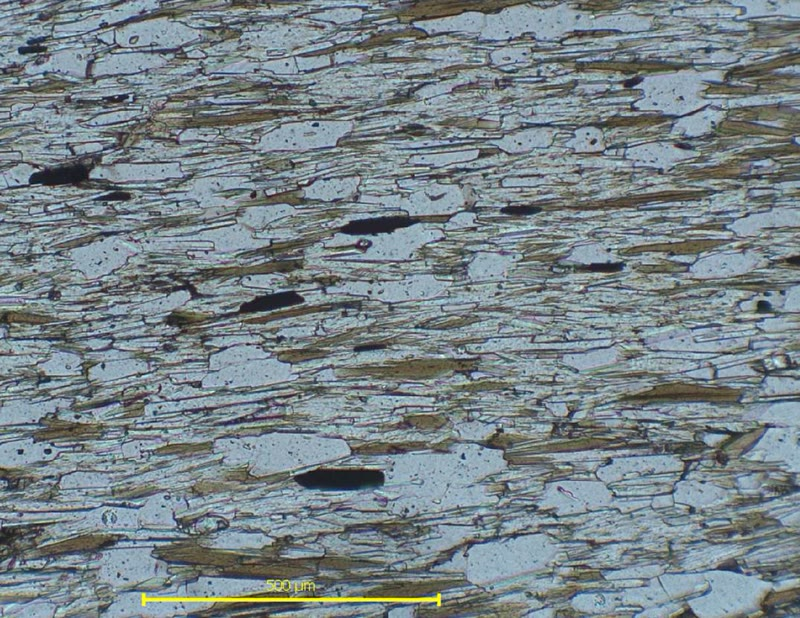
\includegraphics[height=4.3cm]{images/book2/g12-geoloshe-slaty-cleavage.jpg}\hspace{0.03\linewidth}%
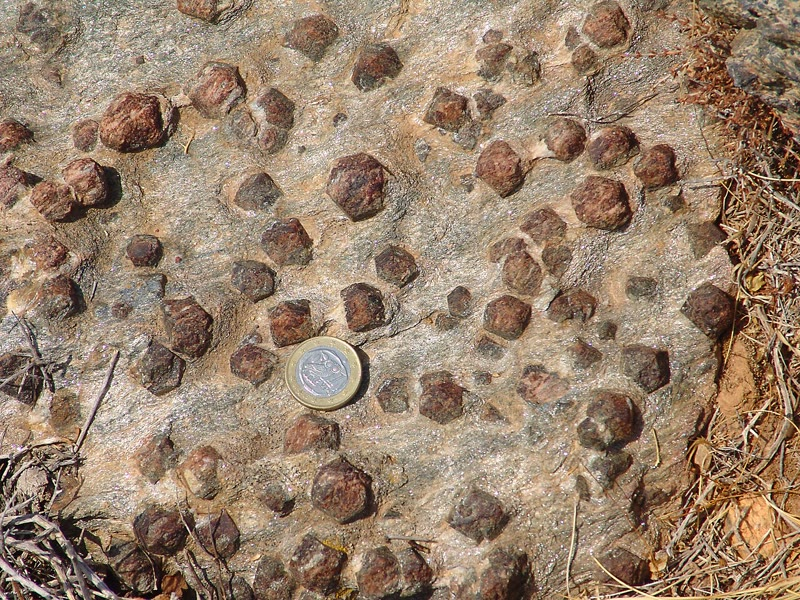
\includegraphics[height=4.3cm]{images/book2/g12-churchard-syros-garnet-schist.jpg}

\smallskip
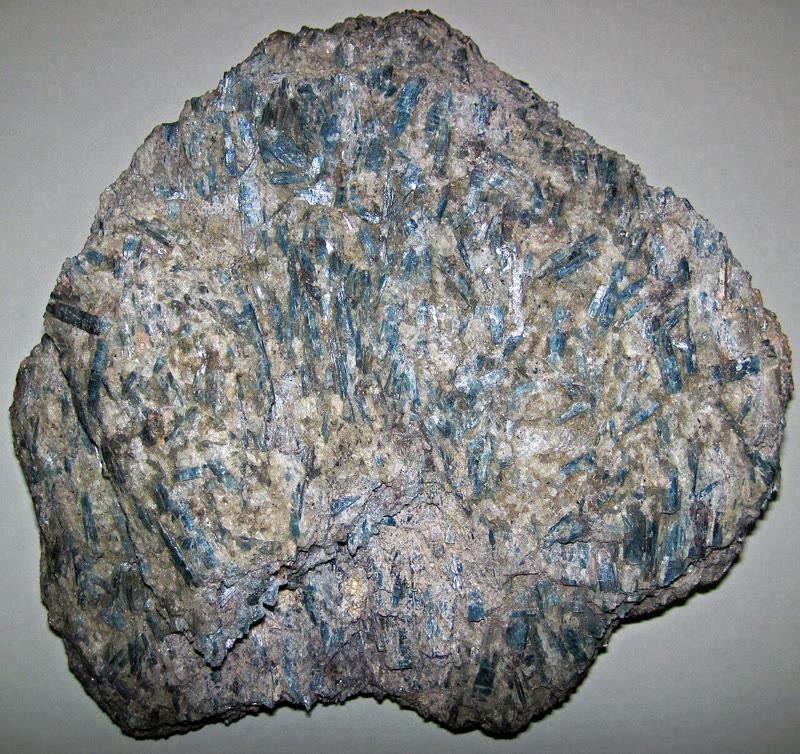
\includegraphics[height=4.3cm]{images/book2/g12-stjohn-kyanite-schist.jpg}\hspace{0.03\linewidth}%
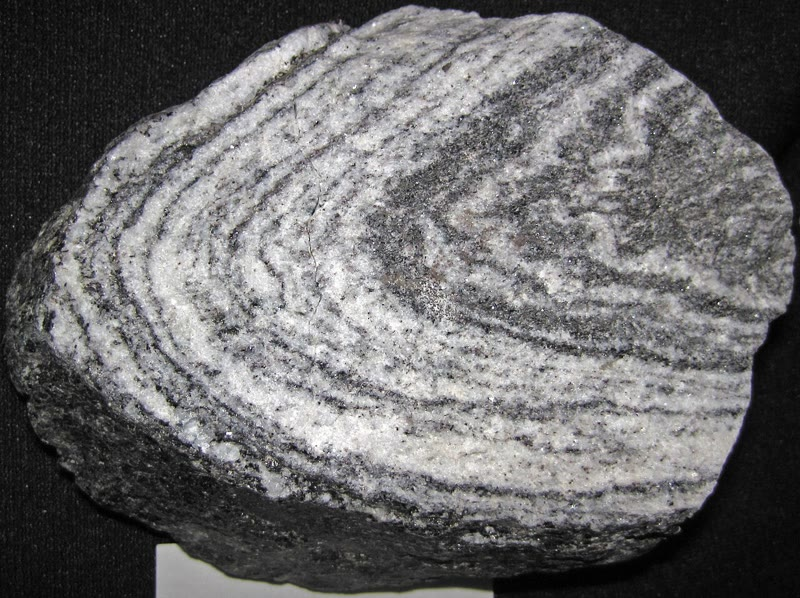
\includegraphics[height=4.3cm]{images/book2/g12-stjohn-gneiss.jpg}

{\small ऊपर बाएँ: सूक्ष्मदर्शी के नीचे एक स्लेट (पीली पट्टी
\qty{500}{\micro\metre} है): उसके अभ्रक के शल्क सब एक ही ओर पड़े हैं।
ऊपर दाएँ: सिरोस द्वीप पर एक गार्नेट-अभ्रक शिस्ट; सिक्का
\qty{23}{mm} चौड़ा है। नीचे बाएँ: कायनाइट के नीले फलकों वाला एक शिस्ट।
नीचे दाएँ: क्वार्ट्ज़ (हल्की) और बायोटाइट अभ्रक (गहरी) की पट्टियों वाला
एक नाइस। फ़ोटो जियोलोशे (CC0), ग्रेम चर्चर्ड (CC~BY~2.0) और जेम्स
सेंट~जॉन (CC~BY~2.0)।}
\end{omfigure}
% ledger: photo:g12-slaty-cleavage, photo:g12-syros-schist, photo:g12-kyanite-schist, photo:g12-gneiss

एक सामान्य \omterm{def:g11:lithosphere-asthenosphere:geotherm}{भूतापीय वक्र} के अनुदिश स्लेट लगभग 5 और \qty{10}{km}
की गहराई के बीच बनती है, फ़िलाइट 10 और 15 के बीच, शिस्ट 15 और 20 के बीच, और नाइस
20 और \qty{25}{km} के बीच; और गहरे में चट्टान कहीं-कहीं पिघलने लगती है।
\omterm{def:g12:metamorphic-rocks:foliation}{पत्रण} भिंचाव की दिशा दर्ज करता है: वह पर्वत बनाने वाले
\omterm{def:g12:mountain-building:shortening}{लघुकरण} के आर-पार बनता है (\cref{ch:g12:mountain-building}), और पंक की
मूल परतें अब भी उसे किसी कोण पर काटती दिख सकती हैं।
% ledger: earle:settings, earle:foliation

जिन चट्टानों में चपटे या लंबे खनिज नहीं होते, वे भींचे जाने पर भी \omterm{def:g12:metamorphic-rocks:foliation}{पत्रण} नहीं
दिखातीं। चूना पत्थर \textbf{संगमरमर} बन जाता है, जो कैल्साइट के बड़े क्रिस्टलों से
बना होता है और जिसमें जीवाश्म मिट चुके होते हैं; बलुआ पत्थर
\textbf{क्वार्टज़ाइट} बन जाता है, जिसके क्वार्ट्ज़ कण बढ़कर एक-दूसरे में घुस गए हैं; और
बिना भींचे गरम हुआ पंक बिना \omterm{def:g12:metamorphic-rocks:foliation}{पत्रण} की एक कठोर, सूक्ष्मकणी चट्टान बन जाता है,
\textbf{हॉर्नफ़ेल्स}।
% ledger: earle:foliation, earle:contact

\section{संस्पर्श और क्षेत्रीय कायांतरण}

\begin{definition}[संस्पर्श कायांतरण; क्षेत्रीय कायांतरण; परिमंडल]\label{def:g12:metamorphic-rocks:contact-regional}
\emph{संस्पर्श कायांतरण}\index{संस्पर्श कायांतरण} उन चट्टानों का \omterm{def:g12:metamorphic-rocks:metamorphism}{कायांतरण} है
जिन्हें उनमें अंतर्वेधित हुए मैग्मा के किसी पिंड ने गरम किया हो; वह
\omterm{def:g11:igneous-rocks:intrusion}{अंतर्वेधन} के चारों ओर के एक क्षेत्र, उसके \emph{परिमंडल}\index{परिमंडल}, तक सीमित रहता है, जिसमें
श्रेणी संपर्क की ओर बढ़ती है। \emph{क्षेत्रीय
कायांतरण}\index{क्षेत्रीय कायांतरण} बड़े प्रदेशों में गहरे दबी चट्टानों को
प्रभावित करता है, सामान्यतः वहाँ जहाँ प्लेटें अभिसरित होती हैं; चट्टानें गरम होने के साथ-साथ
भींची भी जाती हैं, और लगभग सदा पत्रित होती हैं।
\end{definition}
% ledger: earle:contact, earle:regional, tulane:metamorphism

\subsection{मैग्मा के किसी पिंड के चारों ओर}

लगभग \qty{1000}{\celsius} पर मैग्मा का कोई पिंड जो ठंडी ऊपरी
भूपर्पटी में ऊपर उठता है, अपने चारों ओर की चट्टानों को गरम करता है। उनका तापमान 300 से लेकर
\qty{800}{\celsius} से भी अधिक तक पहुँच सकता है, उथली गहराइयों के निम्न दाबों पर।
\omterm{def:g12:metamorphic-rocks:contact-regional}{परिमंडल} संकरा होता है: मैग्मा की किसी पतली चादर के चारों ओर कुछ सेंटीमीटर, किसी बड़े पिंड के चारों ओर
कई दसियों मीटर तक। उसकी चट्टानें बिना
भींचे गरम होती हैं, इसलिए वे पत्रित नहीं होतीं: पंक हॉर्नफ़ेल्स बन जाता है, चूना पत्थर
संगमरमर, बलुआ पत्थर क्वार्टज़ाइट। मैग्मा का जो पिंड पहले से गरम चट्टानों में गहरे
बैठता है, वह लगभग कोई \omterm{def:g12:metamorphic-rocks:contact-regional}{परिमंडल} नहीं बनाता।
% ledger: earle:contact, earle:settings (magma bodies around 1000 degC)

\begin{omfigure}
\begin{tikzpicture}[font=\scriptsize]
  \def\pluton{(3.0,0) .. controls (3.0,2.3) and (7.0,2.3) .. (7.0,0) -- cycle}
  \def\aureole{(2.45,0) .. controls (2.45,2.95) and (7.55,2.95) .. (7.55,0) -- cycle}
  \fill[lith sandstone] (0,0) rectangle (10,0.8);
  \fill[lith limestone] (0,0.8) rectangle (10,1.6);
  \fill[lith shale] (0,1.6) rectangle (10,3);
  \fill[omThm, opacity=0.30] \aureole;
  \draw[omThm, line width=0.6pt, dashed] (2.45,0) .. controls (2.45,2.95) and (7.55,2.95) .. (7.55,0);
  \fill[lith granite] \pluton;
  \draw[black!70, line width=0.6pt] (3.0,0) .. controls (3.0,2.3) and (7.0,2.3) .. (7.0,0);
  \draw[black!60] (0,0) rectangle (10,3);
  \node[fill=white, inner sep=1.5pt] at (5,0.45) {ग्रेनाइट (कभी मैग्मा)};
  \draw[black!70] (6.0,1.95) -- (10.6,2.4) node[right] {हॉर्नफ़ेल्स, पंक से};
  \draw[black!70] (7.0,1.2) -- (10.6,1.2) node[right] {संगमरमर, चूना पत्थर से};
  \draw[black!70] (7.25,0.4) -- (10.6,0.4) node[right] {क्वार्टज़ाइट, बलुआ पत्थर से};
  \node[left] at (0,2.3) {शेल};
  \node[left] at (0,1.2) {चूना पत्थर};
  \node[left] at (0,0.4) {बलुआ पत्थर};
  \draw[omThm] (4.2,2.05) -- (3.4,3.25) node[above, omThm] {परिमंडल};
\end{tikzpicture}

{\small \omterm{def:g12:metamorphic-rocks:contact-regional}{संस्पर्श कायांतरण}, अनुप्रस्थ काट में: मैग्मा का एक पिंड परतदार अवसादी चट्टानों में
ऊपर उठा है और अपने चारों ओर एक संकरे \omterm{def:g12:metamorphic-rocks:contact-regional}{परिमंडल} (लाल) को गरम किया है,
जिसकी चट्टानें बिना भींचे पुनः क्रिस्टलित होती हैं। योजनाबद्ध: वास्तविक \omterm{def:g12:metamorphic-rocks:contact-regional}{परिमंडल}
सेंटीमीटरों से लेकर दसियों मीटर तक चौड़े होते हैं।}
\end{omfigure}
% ledger: earle:contact

\subsection{किसी पर्वत-पट्टी के नीचे}

\omterm{def:g12:metamorphic-rocks:contact-regional}{क्षेत्रीय कायांतरण} के लिए 10 या \qty{20}{km} तक दबना आवश्यक है, इसलिए वह
एक साथ हज़ारों वर्ग किलोमीटर को प्रभावित करता है। इसका सबसे संभावित स्थान किसी
पर्वत-पट्टी का \omterm{def:g12:continental-crust:root}{मूल} है, जहाँ टक्कर भूपर्पटी को मोटा करती है और उसकी चट्टानों को नीचे धकेलती है
(\cref{ch:g12:mountain-building})। एक पुरानी पट्टी में, जिसके क्षेत्रों का
मानचित्र बनाया गया है, सिलिमेनाइट क्षेत्र की चट्टानें
\qty{700}{\celsius} से ऊपर गरम हुईं और 20 से \qty{25}{km} गहरे दबीं, जबकि
बाहरी क्लोराइट क्षेत्र की चट्टानें संभवतः कभी लगभग \qty{5}{km} से अधिक नहीं दबीं।
ऊपर के पर्वत फिर दसियों मिलियन वर्षों में घिस गए; जैसे-जैसे
भार हटा, मोटी भूपर्पटी फिर ऊपर उठी, और कभी गहरे रहे क्षेत्र अब
सतह पर हैं (\cref{ch:g12:destruction-of-mountains})।
% ledger: earle:regional

\subsection{तीन भूतापीय वक्र}

\omterm{def:g12:metamorphic-rocks:polymorph}{बहुरूप} एक नज़र में दिखा देते हैं कि एक ही गहराई का अर्थ हर जगह एक ही
चट्टान नहीं है: वह \omterm{def:g11:lithosphere-asthenosphere:geotherm}{भूतापीय वक्र} पर निर्भर है। \omterm{def:g12:metamorphic-rocks:polymorph}{बहुरूपों} का चित्र
उनमें से तीन दिखाता है।
% ledger: earle:settings

\begin{itemize}
  \item एक \textbf{सामान्य} \omterm{def:g11:lithosphere-asthenosphere:geotherm}{भूतापीय वक्र}, लगभग \qty{30}{\celsius} प्रति
        किलोमीटर: तापमान \qty{10}{km} पर लगभग \qty{300}{\celsius} तक
        पहुँचता है। वह त्रिक बिंदु के नीचे से गुज़रता है, इसलिए कायनाइट
        सीधे सिलिमेनाइट को जगह देता है, लगभग \qty{574}{\celsius} और
        \qty{18.8}{km} पर।
  \item किसी \textbf{ज्वालामुखीय क्षेत्र} का \omterm{def:g11:lithosphere-asthenosphere:geotherm}{भूतापीय वक्र}, 40 से \qty{50}{\celsius} प्रति
        किलोमीटर, जिसे ऊपर उठते मैग्मा की ऊष्मा ने अधिक खड़ा कर दिया है: चट्टानें
        उथली गहराइयों पर ऊँचे तापमानों तक पहुँचती हैं। \qty{50}{\celsius} प्रति
        किलोमीटर पर ऐंडालुसाइट लगभग \qty{6.6}{km} पर प्रकट होता है और
        लगभग \qty{10.9}{km}, \qty{553}{\celsius}, पर सिलिमेनाइट को जगह देता है।
  \item किसी \textbf{\omterm{def:g11:subduction-zones:subduction}{क्षेपण क्षेत्र}} का \omterm{def:g11:lithosphere-asthenosphere:geotherm}{भूतापीय वक्र}, प्रति किलोमीटर
        \qty{10}{\celsius} से कम: नीचे ले जाई गई \omterm{def:g11:ocean-ridges:oceanic-lithosphere}{महासागरीय भूपर्पटी}
        अपने चारों ओर के प्रावार से कई सौ अंश ठंडी रहती है।
        \qty{36}{km} पर वह केवल लगभग \qty{370}{\celsius} पर है, कायनाइट
        क्षेत्र के भीतर गहरे। यह वह ठंडा, ऊँचे दाब वाला पथ है जिस पर बेसाल्ट
        लगभग \qty{35}{km} पर \omterm{def:g11:subduction-zones:eclogite}{नीलशिस्ट}, फिर \omterm{def:g11:subduction-zones:eclogite}{एक्लोजाइट} बन जाता है।
\end{itemize}
% values: cross_30_0 573.6 degC 18.79 km; cross_50_0 340.1 degC 6.60 km; cross_50_1 553.0 degC 10.86 km; sub10_T_at_1gpa 370.2 (al2sio5.py)
% ledger: earle:settings

इस तरह हर कायांतरित चट्टान उस \omterm{def:g11:lithosphere-asthenosphere:geotherm}{भूतापीय वक्र} का अभिलेख रखती है जिसके अंतर्गत वह
बनी, और उसके पीछे की प्लेट-स्थिति का भी: ऐंडालुसाइट और हॉर्नफ़ेल्स
उथली गहराइयों पर, मैग्मा के पिंडों के चारों ओर, ऊष्मा की ओर संकेत करते हैं; कायनाइट और सिलिमेनाइट
वाले शिस्ट और नाइस पर्वत-पट्टियों के गहरे \omterm{def:g12:continental-crust:root}{मूलों} की ओर; \omterm{def:g11:subduction-zones:eclogite}{नीलशिस्ट} और
\omterm{def:g11:subduction-zones:eclogite}{एक्लोजाइट} \omterm{def:g11:subduction-zones:subduction}{क्षेपण क्षेत्रों} की ओर। इनमें से अधिकांश चट्टानें केवल इसलिए देखी जा सकीं
क्योंकि वे वापस बदले बिना सतह पर लौट आईं। ऊपर उठते और
ठंडे होते हुए उनकी अभिक्रियाएँ धीमी हो जाती हैं, और उलटी
अभिक्रियाओं को जिस जल की आवश्यकता होती, वह नीचे जाते समय ही निकल चुका होता है।
% ledger: earle:settings, earle:contact, tulane:metamorphism (retrograde metamorphism uncommon)

\section{अभ्यास}

\begin{exercise}[$\star$]\label{exo:g12:metamorphic-rocks:1}
शब्द बताइए: (a) एक ही संघटन पर भिन्न क्रिस्टल
संरचनाओं वाले खनिज; (b) मानचित्र पर वह रेखा जहाँ कोई \omterm{def:g12:metamorphic-rocks:index-mineral}{सूचक खनिज} पहली बार प्रकट होता है;
(c) मैग्मा के किसी पिंड के चारों ओर गरम हुई चट्टानों का क्षेत्र; (d) एक सीध में आए चपटे
खनिजों से बने समांतर तल; (e) ऊपर की चट्टानों के भार के कारण
दाब।
\end{exercise}

\begin{exercise}[$\star$]\label{exo:g12:metamorphic-rocks:2}
हर \omterm{def:g10:soil-formation:weathering-profile}{जनक चट्टान} जिस कायांतरित चट्टान में बदलती है, उसका नाम बताइए: (1) चूना पत्थर;
(2) बलुआ पत्थर; (3) पंक, भिंचाव के अंतर्गत निम्न श्रेणी पर; (4) पंक, उच्च
श्रेणी पर; (5) पंक, जिसे मैग्मा के किसी पिंड ने बिना भींचे गरम किया हो।
\end{exercise}

\begin{exercise}[$\star$]\label{exo:g12:metamorphic-rocks:3}
$\rho = \qty{2830}{kg/m^3}$ और $g = \qty{9.81}{m/s^2}$ के साथ,
\qty{10}{km} और \qty{20}{km} पर \omterm{def:g12:metamorphic-rocks:lithostatic}{शैलस्थैतिक दाब} \unit{GPa} में परिकलित कीजिए।
\end{exercise}

\begin{exercise}[$\star$]\label{exo:g12:metamorphic-rocks:4}
\ce{Al2SiO5} के \omterm{def:g12:metamorphic-rocks:polymorph}{बहुरूपों} के आरेख पर कौन-सा खनिज स्थायी है:
(1) \qty{400}{\celsius} और \qty{0.6}{GPa} पर; (2) \qty{500}{\celsius}
और \qty{0.2}{GPa} पर; (3) \qty{750}{\celsius} और \qty{0.3}{GPa} पर?
\end{exercise}

\begin{exercise}[$\star$]\label{exo:g12:metamorphic-rocks:5}
(1) बढ़ती श्रेणी के क्रम में रखिए: शिस्ट, स्लेट, नाइस, फ़िलाइट। (2) इनमें से
किसमें अभ्रक नंगी आँख से देखे जा सकते हैं? (3) कौन-सी
हल्की और गहरी पट्टियाँ दिखाती है?
\end{exercise}

\begin{exercise}[$\star\star$]\label{exo:g12:metamorphic-rocks:6}
(1) \qty{35}{km} मोटी भूपर्पटी के आधार पर \omterm{def:g12:metamorphic-rocks:lithostatic}{शैलस्थैतिक दाब} परिकलित कीजिए
($\rho = \qty{2830}{kg/m^3}$) और उसे वायुमंडल में व्यक्त कीजिए
($\qty{1}{atm} = \qty{101325}{Pa}$)। (2) \qty{4}{km} गहरे महासागर की तली पर
दाब परिकलित कीजिए, समुद्री जल का घनत्व
\qty{1025}{kg/m^3} लेकर। (3) पहला कितने गुना बड़ा है?
\end{exercise}

\begin{exercise}[$\star\star$]\label{exo:g12:metamorphic-rocks:7}
\ce{Al2SiO5} का त्रिक बिंदु \qty{504}{\celsius} और
\qty{0.375}{GPa} पर है। (1) वह दाब किस गहराई पर पहुँचता है ($\rho =
\qty{2830}{kg/m^3}$)? (2) सतह पर \qty{10}{\celsius} से शुरू होने वाली कौन-सी
\omterm{def:g11:lithosphere-asthenosphere:geotherm}{भूतापीय प्रवणता} ठीक उससे होकर गुज़रती है? (3) क्या तीनों \omterm{def:g12:metamorphic-rocks:polymorph}{बहुरूप} रखने वाली चट्टान
के आम होने की संभावना है?
\end{exercise}

\begin{exercise}[$\star\star$]\label{exo:g12:metamorphic-rocks:8}
सिरोस के गार्नेट शिस्ट की फ़ोटो में सबसे बड़े गार्नेट
सिक्के के लगभग एक-तिहाई चौड़े हैं, जो \qty{23}{mm} है। (1) उनके
व्यास का अनुमान लगाइए। (2) यदि किसी गार्नेट का व्यास एक मिलियन वर्ष में लगभग \qty{1}{mm}
बढ़ता है, तो उन्हें बढ़ने में कितना समय लगा? (3) इससे आपको किसी
चट्टान के गहराई में बिताए समय के बारे में क्या पता चलता है?
\end{exercise}

\begin{exercise}[$\star\star$]\label{exo:g12:metamorphic-rocks:9}
किसी पुरानी पर्वत-पट्टी के आर-पार \qty{24}{km} पश्चिम की ओर चलते हुए एक भूवैज्ञानिक
पंक से बनी चट्टानें दर्ज करती है। शुरुआत में उनमें केवल क्लोराइट और बायोटाइट
हैं; पहला गार्नेट \qty{6}{km} के बाद प्रकट होता है, पहला स्टॉरोलाइट
\qty{11}{km} के बाद, पहला कायनाइट \qty{15}{km} के बाद, पहला सिलिमेनाइट
\qty{20}{km} के बाद। (1) कितनी \omterm{def:g12:metamorphic-rocks:index-mineral}{समश्रेणी-रेखाएँ} पार की गईं? उनके नाम क्रम से बताइए।
(2) श्रेणी किस दिशा में बढ़ती है? (3) चट्टानें सबसे गहरी कहाँ दबी थीं,
और वहाँ वे मोटे तौर पर कितनी गरम हुईं?
\end{exercise}

\begin{exercise}[$\star\star$]\label{exo:g12:metamorphic-rocks:10}
मैग्मा का एक पिंड सतह के निकट पंक, चूना पत्थर और बलुआ पत्थर की परतों में ऊपर उठता है।
(1) उसके पास हर परत जिस चट्टान में बदलती है, उसका नाम बताइए। (2) ये
चट्टानें पत्रित क्यों नहीं हैं? (3) मैग्मा का एक दूसरा पिंड \qty{20}{km} नीचे,
पहले से लगभग \qty{500}{\celsius} की चट्टानों में, बैठता है। वह लगभग कोई \omterm{def:g12:metamorphic-rocks:contact-regional}{परिमंडल} क्यों नहीं बनाता?
\end{exercise}

\begin{exercise}[$\star\star$]\label{exo:g12:metamorphic-rocks:11}
किसी टक्कर के दौरान पंक की एक परत पूर्व और पश्चिम से भींची जाती है,
और गरम होते हुए अभ्रक उगाती है। (1) अभ्रक कैसे पड़े होते हैं: उनके चपटे फलक
पूर्व--पश्चिम की ओर मुख किए या उत्तर--दक्षिण की ओर? (2) बनने वाला \omterm{def:g12:metamorphic-rocks:foliation}{पत्रण}
क्षैतिज है या ऊर्ध्वाधर? (3) उसी ढंग से भींचे गए संगमरमर और क्वार्टज़ाइट
कोई \omterm{def:g12:metamorphic-rocks:foliation}{पत्रण} नहीं दिखाते। क्यों?
\end{exercise}

\begin{exercise}[$\star\star\star$]\label{exo:g12:metamorphic-rocks:12}
500 और \qty{700}{\celsius} के बीच कायनाइट--सिलिमेनाइट सीमा
सीधी रेखा $P = 0.577 + 0.00209\,(T - 600)$ के निकट है, जहाँ $P$
\unit{GPa} में और $T$ \unit{\celsius} में है। एक सामान्य \omterm{def:g11:lithosphere-asthenosphere:geotherm}{भूतापीय वक्र} $T = 10 + 30z$ है
($z$ \unit{km} में), और $P = 0.0278\,z$। (1) \omterm{def:g11:lithosphere-asthenosphere:geotherm}{भूतापीय वक्र} को $P$ के रूप में,
$T$ के फलन की तरह, लिखिए। (2) ज्ञात कीजिए कि वह सीमा को कहाँ पार करता है: तापमान, दाब,
गहराई। (3) इस \omterm{def:g11:lithosphere-asthenosphere:geotherm}{भूतापीय वक्र} के अनुदिश उस गहराई से ठीक ऊपर कौन-सा \omterm{def:g12:metamorphic-rocks:polymorph}{बहुरूप} स्थायी है,
और ठीक नीचे कौन-सा?
\end{exercise}

\begin{exercise}[$\star\star\star$]\label{exo:g12:metamorphic-rocks:13}
(1) प्रति किलोमीटर \qty{10}{\celsius} के \omterm{def:g11:subduction-zones:subduction}{क्षेपण} \omterm{def:g11:lithosphere-asthenosphere:geotherm}{भूतापीय वक्र} के अनुदिश,
\qty{10}{\celsius} से शुरू करके, \qty{35}{km} पर, जहाँ
\omterm{def:g11:subduction-zones:eclogite}{एक्लोजाइट} बनता है, तापमान क्या है? (2) प्रति किलोमीटर \qty{30}{\celsius} के
सामान्य \omterm{def:g11:lithosphere-asthenosphere:geotherm}{भूतापीय वक्र} के अनुदिश वह क्या है? (3) दोनों बिंदुओं को \omterm{def:g12:metamorphic-rocks:polymorph}{बहुरूपों} के
आरेख पर रखिए: पहले बिंदु पर कौन-सा \omterm{def:g12:metamorphic-rocks:polymorph}{बहुरूप} स्थायी है? (4) \omterm{def:g11:subduction-zones:eclogite}{नीलशिस्ट} और
\omterm{def:g11:subduction-zones:eclogite}{एक्लोजाइट} \omterm{def:g11:subduction-zones:subduction}{क्षेपण क्षेत्रों} में ही क्यों बनते हैं और लगभग कहीं और क्यों नहीं?
\end{exercise}

\begin{exercise}[$\star\star\star$]\label{exo:g12:metamorphic-rocks:14}
कायनाइट, सिलिमेनाइट और ऐंडालुसाइट के घनत्व \num{3.61},
\num{3.24} और \qty{3.15}{g/cm^3} हैं। (1) हर एक के \qty{1}{kg} का
आयतन \unit{cm^3} में परिकलित कीजिए। (2) समान द्रव्यमान के ऐंडालुसाइट से कायनाइट
कितने प्रतिशत छोटा है? (3) इस विचार से कि ऊँचा दाब उस व्यवस्था के पक्ष में
होता है जो सबसे कम जगह लेती है, समझाइए कि कायनाइट आरेख के
ऊँचे दाब वाले क्षेत्र पर अधिकार क्यों रखता है।
\end{exercise}

\begin{exercise}[$\star\star\star$]\label{exo:g12:metamorphic-rocks:15}
किसी पुरानी पर्वत-पट्टी में सिलिमेनाइट क्षेत्र की चट्टानें
\qty{700}{\celsius} से ऊपर गरम हुईं और 20 से \qty{25}{km} गहरे दबीं। (1) 20 और
\qty{25}{km} पर दाब परिकलित कीजिए। (2) अभ्यास~12 की रेखा का उपयोग करके
इनमें से हर दाब पर वह न्यूनतम तापमान ज्ञात कीजिए जिस पर सिलिमेनाइट स्थायी है।
क्या \qty{700}{\celsius} सिलिमेनाइट से संगत है?
(3) सतह पर \qty{10}{\celsius} से शुरू करके, 20 और \qty{25}{km} पर
\qty{700}{\celsius} कौन-सी \omterm{def:g11:lithosphere-asthenosphere:geotherm}{भूतापीय प्रवणताएँ} दर्शाता है? (4) चट्टानें
लगभग 40 मिलियन वर्ष बाद सतह पर अनावृत हुईं। उनके ऊपर की चट्टान किस माध्य दर से
हटाई गई, \unit{mm} प्रति वर्ष में?
\end{exercise}

\begin{problem}[{सप्ताहांत समस्या --- एक कायनाइट शिस्ट का इतिहास}]
\label{pb:g12:metamorphic-rocks:1}
% ledger: hm93:table11, cm95:crust, earle:controls, earle:settings, earle:regional, tulane:roots, tulane:metamorphism, iugs:barrow; Book 3: webmineral:polymorphs; Book 1: ussa76:sea-level
% values: pb_z_km 25.214, pb_grad 23.4, pb_kysil_P_at_600_gpa 0.577 (al2sio5.py); t_on_kysil(7.0) = 658.9
किसी पुरानी पर्वत-पट्टी के क्रोड से एकत्र किए गए एक शिस्ट में मस्कोवाइट,
बायोटाइट, क्वार्ट्ज़, \qty{8}{mm} तक चौड़े गार्नेट, और कायनाइट के नीले
फलक हैं; उसमें न सिलिमेनाइट है, न ऐंडालुसाइट। उसके गार्नेट और बायोटाइट के
प्रयोगशाला-विश्लेषण उन परिस्थितियों को बताते हैं जिनमें वह क्रिस्टलित हुआ:
लगभग \qty{600}{\celsius} और \qty{0.70}{GPa}। $\rho =
\qty{2830}{kg/m^3}$, $g = \qty{9.81}{m/s^2}$, सतह पर \qty{10}{\celsius},
और अभ्यास~12 की कायनाइट--सिलिमेनाइट रेखा, $P = 0.577 +
0.00209\,(T - 600)$, लीजिए।

\medskip
\noindent\textbf{भाग I --- खनिज।}
\begin{enumerate}
  \item इस चट्टान को शिस्ट क्यों कहा जाता है? उसके कौन-से खनिज
        \omterm{def:g12:metamorphic-rocks:foliation}{शिस्टाभता} बनाते हैं?
  \item कायनाइट, ऐंडालुसाइट और सिलिमेनाइट का सूत्र एक ही है। उसे लिखिए, और
        ऐसे खनिजों के लिए शब्द बताइए।
  \item कायनाइट और ऐंडालुसाइट के घनत्व \num{3.61} और
        \qty{3.15}{g/cm^3} हैं। एक किलोग्राम कायनाइट का आयतन कितने प्रतिशत
        छोटा है? दाब किसके पक्ष में होता है?
  \item पंक से बनी चट्टानों के \omterm{def:g12:metamorphic-rocks:index-mineral}{सूचक खनिजों} के अनुक्रम में यह चट्टान किस क्षेत्र
        की है? नीचे जाते हुए उसने कौन-सी \omterm{def:g12:metamorphic-rocks:index-mineral}{समश्रेणी-रेखाएँ} पार कीं?
  \item यदि गार्नेटों का व्यास एक मिलियन वर्ष में लगभग \qty{1}{mm}
        बढ़ा, तो सबसे बड़े गार्नेटों को बढ़ने में कितना समय लगा?
\end{enumerate}

\medskip
\noindent\textbf{भाग II --- दाब और तापमान।}
\begin{enumerate}[resume]
  \item \qty{600}{\celsius} पर, किस दाब से ऊपर सिलिमेनाइट के बजाय कायनाइट
        स्थायी है?
  \item जाँचिए कि बिंदु (\qty{600}{\celsius}, \qty{0.70}{GPa})
        कायनाइट क्षेत्र में पड़ता है।
  \item अनुपस्थित सिलिमेनाइट \qty{600}{\celsius} पर एक न्यूनतम
        दाब देता है। वह क्या है?
  \item यदि चट्टान को \qty{0.70}{GPa} पर और गरम किया गया होता, तो किस
        तापमान पर उसका कायनाइट सिलिमेनाइट में बदल जाता?
  \item \qty{0.70}{GPa} को किलोबार ($\qty{1}{kbar} =
        \qty{e8}{Pa}$) और वायुमंडल ($\qty{1}{atm} = \qty{101325}{Pa}$) में व्यक्त कीजिए।
\end{enumerate}

\medskip
\noindent\textbf{भाग III --- दबने की गहराई।}
\begin{enumerate}[resume]
  \item \omterm{def:g12:metamorphic-rocks:lithostatic}{शैलस्थैतिक दाब} प्रति किलोमीटर कितने मेगापास्कल
        बढ़ता है?
  \item क्रिस्टलित होते समय शिस्ट किस गहराई पर था?
  \item अनुपस्थित सिलिमेनाइट द्वारा अनुमत सबसे कम गहराई क्या है
        (प्रश्न 8)?
  \item ऊपर की चट्टानों के लिए \qty{2700}{kg/m^3} घनत्व लेकर प्रश्न 12 फिर से कीजिए।
        गहराई कितने प्रतिशत बदलती है?
  \item \omterm{def:g12:continental-crust:continental-crust}{महाद्वीपीय भूपर्पटी} सामान्यतः 35 से \qty{40}{km} मोटी होती है, और
        पर्वत-पट्टियों के नीचे 50 से \qty{70}{km}। शिस्ट
        भूपर्पटी में क्रिस्टलित हुआ या प्रावार में?
\end{enumerate}

\medskip
\noindent\textbf{भाग IV --- भूतापीय वक्र, और ऊपर लौटने का रास्ता।}
\begin{enumerate}[resume]
  \item उस गहराई पर \qty{600}{\celsius} कौन-सी माध्य \omterm{def:g11:lithosphere-asthenosphere:geotherm}{भूतापीय प्रवणता}
        दर्शाता है?
  \item इसकी तुलना किसी \omterm{def:g11:subduction-zones:subduction}{क्षेपण क्षेत्र}, किसी सामान्य भूपर्पटी और किसी ज्वालामुखीय
        क्षेत्र की प्रवणताओं से कीजिए। किस प्रकार के \omterm{def:g12:metamorphic-rocks:metamorphism}{कायांतरण} ने यह चट्टान बनाई?
  \item प्रति किलोमीटर \qty{30}{\celsius} के सामान्य \omterm{def:g11:lithosphere-asthenosphere:geotherm}{भूतापीय वक्र} के अनुदिश, प्रश्न 12 की
        गहराई पर तापमान क्या होता? तब \qty{0.70}{GPa} पर कौन-सा
        \omterm{def:g12:metamorphic-rocks:polymorph}{बहुरूप} स्थायी होता?
  \item शिस्ट को सतह पर लाने के लिए उसके ऊपर की सारी चट्टान को हटना
        पड़ा। प्रति वर्ष \qty{0.5}{mm} की माध्य दर से इसमें कितना समय
        लगा?
  \item ऊपर आते हुए कायनाइट वापस ऐंडालुसाइट में क्यों नहीं बदला?
  \item सारांश दीजिए: यह कायनाइट शिस्ट किस गहराई पर क्रिस्टलित हुआ?
\end{enumerate}
\end{problem}
